\documentclass[12pt,a4paper]{report}

%----------------------------------------------------------
%Thiết lập lề trang giấy
\usepackage{anysize}
\marginsize{3.0 cm}{2.5 cm}{1.5 cm}{1.5 cm}

%----------------------------------------------------------
%Lùi đầu dòng cho đoạn đầu tiên của một mục
\usepackage{indentfirst}
%----------------------------------------------------------
%Thiết lập khoảng cách giữa các dòng và các đoạn

%----------------------------------------------------------
%Sử dụng font Unicode cho tiếng Việt
\usepackage[utf8]{vietnam}

%----------------------------------------------------------
%Sử dụng các font toán học
\usepackage{latexsym}
\usepackage{amssymb}
%\usepackage{amsthm}
%----------------------------------------------------------
\usepackage{stmaryrd}
\usepackage{url}
\usepackage[all]{xy}
\usepackage{xspace}
\usepackage[ruled,vlined,linesnumbered]{algorithm2e}
\usepackage{graphicx}
%----------------------------------------------------------
\usepackage{algorithmic}
\usepackage{array}
\usepackage{mdwmath}
\usepackage[cmex10]{amsmath}
\usepackage{mdwtab}
\usepackage{eqparbox}
\usepackage[caption=false,font=footnotesize]{subfig}
\usepackage{fixltx2e}
%----------------------------------------------------------
%Dùng cho bảng biểu
\usepackage{tabularx}
\usepackage{longtable}
%----------------------------------------------------------
%Định dạng chương, định lý, mệnh đề, ...
\newtheorem{Chapter}{Chương}
\newtheorem{Definition}{Định nghĩa}[chapter]
\newtheorem{Theorem}{Định lý}[chapter]
\newtheorem{Proposition}{Mệnh đề}[chapter]
\newtheorem{Lemma}{Bổ đề}[chapter]
\newtheorem{Corollary}{Hệ quả}[chapter]
\newtheorem{Remark}{Ghi chú}[chapter]
\newtheorem{Example}{Ví dụ}[chapter]

\newenvironment{definition}
{\
  \smallskip
  \begin{Definition} 
    \begin{em}}
    {\end{em}
  \end{Definition}
  \smallskip
}

\newenvironment{theorem}
{
  \smallskip
  \begin{Theorem}
    \begin{em}}
    {\end{em}
  \end{Theorem}
  \smallskip
}

\newenvironment{proposition}
{
  \smallskip
  \begin{Proposition}
    \begin{em}}
    {\end{em}
  \end{Proposition}
  \smallskip
}

\newenvironment{lemma}
{
  \smallskip
  \begin{Lemma}
    \begin{em}}
    {\end{em}
  \end{Lemma}
  \smallskip
}

\newenvironment{corollary}
{
  \smallskip
  \begin{Corollary}
    \begin{em}}
    {\end{em}
  \end{Corollary}
  \smallskip
}

\newenvironment{remark}
{
  \smallskip
  \begin{Remark}
    \begin{em}}
    {\end{em}
  \end{Remark}
  \smallskip
}

\newenvironment{example}
{
  \smallskip
  \begin{Example}
    \begin{em}}
    {\end{em}
  \end{Example}
  \smallskip
}

\newcommand{\myend}{\mbox{}\hfill\mbox{{\scriptsize$\!\blacksquare$}}}
\newenvironment{sketch}{\noindent{\em Proof sketch.}}{\myend\smallskip}
\newcommand{\HRule}{\rule{\linewidth}{0.6mm}}

%--------------------------------------------------------------

\newcommand{\mand}{\sqcap}
\newcommand{\mor}{\sqcup}
\newcommand{\V}{\forall}
\newcommand{\E}{\exists}

%--------------------------------------------------------------
%Định nghĩa các ký hiệu viết tắt cho logic mô tả
\newcommand{\AL}{$\mathcal{AL}$}
\newcommand{\ALC}{$\mathcal{ALC}$}
\newcommand{\ALCI}{$\mathcal{ALCI}$}
\newcommand{\ALCQ}{$\mathcal{ALCQ}$}
\newcommand{\ALCIQ}{$\mathcal{ALCIQ}$}
\newcommand{\ALCN}{$\mathcal{ALCN}$}
\newcommand{\LogicS}{$\mS$}
\newcommand{\SI}{$\mathcal{SI}$}
\newcommand{\SH}{$\mathcal{SH}$}
\newcommand{\SHI}{$\mathcal{SHI}$}
\newcommand{\SHIQ}{$\mathcal{SHIQ}$}
\newcommand{\SHOIQ}{$\mathcal{SHOIQ}$}
\newcommand{\SHIN}{$\mathcal{SHIN}$}
\newcommand{\SHOIN}{$\mathcal{SHOIN}$}

\newcommand{\mL}{\mathcal{L}}
\newcommand{\mG}{\mathcal{G}}
\newcommand{\mT}{\mathcal{T}}
\newcommand{\mA}{\mathcal{A}}
\newcommand{\mI}{\mathcal{I}}
\newcommand{\mC}{\mathcal{C}}
\newcommand{\mE}{\mathcal{E}}
\newcommand{\mS}{\mathcal{S}}


\newcommand{\EXPTIME}{{\sc ExpTime}\xspace}
\newcommand{\NEXPTIME}{{\sc NExpTime}\xspace}
\newcommand{\ptime}{{\sc PTime}\xspace}
%-----------------------------------------------------------------
\renewcommand{\baselinestretch}{1.3}
%-----------------------------------------------------------------
%Định nghĩa tuple <>
\def\tuple#1{\left\langle#1\right\rangle}

%-----------------------------------------------------------------

\begin{document}

\begin{titlepage}
\begin{center}
%\includegraphics[width=0.15\textwidth]{./logo}\\[1cm]    

\textsc{\textbf{ĐẠI HỌC HUẾ}}\\[0.0cm]
{\textbf{TRƯỜNG ĐẠI HỌC KHOA HỌC}}\\[4.5cm]

\textsc{\Large \textbf{BÁO CÁO KẾT QUẢ}}\\
(\textit{Theo hợp đồng số 03/HĐ-NCKH, ngày 02/5/2103})\\[0.3cm]
% Title
\HRule \\[0.6cm]
{ \LARGE \bfseries MỘT SỐ KIẾN THỨC CƠ BẢN VỀ LOGIC MÔ TẢ}\\[0.4cm]
\HRule \\[0.1cm]
\textbf{ĐỀ TÀI: HỌC KHÁI NIỆM ĐỐI VỚI CÁC CƠ SỞ TRI THỨC TRONG LOGIC MÔ TẢ DỰA VÀO MÔ PHỎNG HAI CHIỀU}\\
\textbf{Mã số: DHH2013-01-41}
\\[1.5cm]
% Author and supervisor
\begin{minipage}{0.4\textwidth}
\begin{flushleft} \large
\emph{Chủ nhiệm đề tài}\\
\textsc{Trần Thanh Lương}
\end{flushleft}
\end{minipage}
\begin{minipage}{0.5\textwidth}
\begin{flushright} \large
\emph{Người thực hiện} \\
\textsc{Trương Văn Quốc Nhật}
\end{flushright}
\end{minipage}

\vfill
% Bottom of the page
Huế, 11/2013

\end{center}
\end{titlepage}
\pagenumbering{roman}
\tableofcontents

\pagebreak[4]
\pagenumbering{arabic}

\chapter{Giới thiệu}\label{ch:Introduction}
Logic mô tả (Description Logics - DLs) là một họ các ngôn ngữ hình thức được sử dụng để biểu diễn và suy luận tri thức trong một miền ứng dụng cụ thể. Bắt đầu từ các khái niệm nguyên tử, vai trò nguyên tử, logic mô tả cho phép xây dựng các khái niệm phức, vai trò phức bằng cách sử dụng các khái niệm nguyên tử, vai trò nguyên tử cùng với tập các tạo tử đã cho. Một hệ thống logic mô tả cho phép mô tả các khái niệm có liên quan với nhau và các tri thức tiềm ẩn. Các tri thức tiềm ẩn này có thể được suy luận từ những tri thức đã được biểu diễn thông qua các dịch vụ suy luận hoặc các bộ suy luận.

Trong tiểu luận này, chúng tôi chủ yếu giới thiệu logic mô tả cơ bản nhất đó là logic \ALC\ và các thuật toán suy luận trên logic mô tả \ALC. Ngoài ra, chúng tôi cũng đề cập đến một số logic mô tả mở rộng từ logic mô tả \ALC\ như: \ALCI, \ALCQ, \ALCIQ, \ALCN, \LogicS, \SH, \SHI, \SHIQ, \ldots.
 
\section{Hệ thống logic mô tả}\label{sec:DLSystems}
Thuật ngữ {\em Logic mô tả}, được sử dụng rộng rãi từ năm 1984. Ban đầu logic mô tả được sử dụng để biểu diễn tri thức bởi Quillian vào năm 1967 thông qua thuật ngữ \textit{mạng ngữ nghĩa} (semantic networks) và Minsky vào năm 1981 với thuật ngữ \textit{hệ thống khung} (frame systems). Năm 1985, hệ thống \textsc{KL-one}~\cite{ref:Brachman} ra đời đã đưa ra một định hướng nghiên cứu cho logic mô tả. 

Logic mô tả dựa vào tập ký hiệu các tên cá thể (có thể hiểu như là các đối tượng), tên khái niệm (có thể hiểu như là các lớp, các vị từ một đối), các tên vai trò (có thể hiểu như là các quan hệ hai ngôi, các vị từ hai đối) và tập các tạo tử đặc trưng cho phép tạo nên các khái niệm phức, vai trò phức từ các khái niệm nguyên tử (\textit{bao gồm khái niệm nguyên thủy và khái niệm định nghĩa}) và vai trò nguyên tử (\textit{bao gồm vai trò nguyên thủy và vai trò định nghĩa}).

\begin{Example}\label{ex:PrimitiveConcept}
Giả sử chúng ta có các khái niệm nguyên thủy và vai trò nguyên thủy sau:

  \begin{tabular}{l l}
   $\mathsf{Human}$ & là khái niệm để chỉ các đối tượng là người\\
   $\mathsf{Female}$ & là khái niệm để chỉ các đối tượng là giống cái\\
%   $\mathsf{Male}$ & là khái niệm để chỉ các đối tượng là giống đực\\
   $\mathsf{Rich}$ & là khái niệm để chỉ những đối tượng giàu có\\
   $\mathsf{hasChild}$ & là vai trò để chỉ đối tượng này có con là đối tượng kia\\
   $\mathsf{marriedTo}$ & là vai trò để chỉ đối tượng này kết hôn với đối tượng kia \hspace{10.5ex} \myend
  \end{tabular}
\end{Example}

\begin{Example}
Với những khái niệm nguyên thủy, vai trò nguyên thủy đã cho trong Ví dụ~\ref{ex:PrimitiveConcept} và các tạo tử \textit{phủ định của khái niệm} ($\neg$), \textit{giao của các khái niệm} ($\mand$), \textit{hợp của các khái niệm} ($\mor$), \textit{lượng từ hạn chế tồn tại} ($\E$), \textit{lượng từ hạn chế với mọi} ($\V$), chúng ta có thể xây dựng các khái niệm phức sau:

  \begin{tabular}{l}
%    \hline   
    $\mathsf{Human \mand Female}$\\
    \qquad là khái niệm để chỉ các đối tượng là người phụ nữ\\
    $\mathsf{Human \mand \neg Female}$\\
    \qquad là khái niệm để chỉ các đối tượng là người đàn ông\\
    $\mathsf{Human \mand \E hasChild.(Human \mand Female)}$\\
    \qquad là khái niệm để chỉ các đối tượng là cha mẹ có con gái\\
    $\mathsf{Human \mand \E marriedTo.Human}$\\
    \qquad là khái niệm để chỉ những người đã kết hôn\\ 
    $\mathsf{Human \mand \V hasChild.Female}$\\
    \qquad là khái niệm để chỉ những người chỉ có toàn con gái\\
    $\mathsf{Female \mand Rich}$\\
    \qquad là khái niệm để chỉ những phụ nữ giàu có \hspace{31.5ex} \myend
%    \hline
  \end{tabular}
\end{Example}

Từ các tên cá thể, khái niệm và vai trò, người ta có thể xây dựng một hệ thống logic mô tả và được gọi là một hệ cơ sở tri thức để thực hiện việc biểu diễn thông tin và suy luận. Thông thường, một cơ sở tri thức gồm có các thành phần sau~\cite{ref:Baader00}:

\begin{figure}[h]
  \setlength{\unitlength}{1cm}
  \begin{picture}(15, 5.5)(0,0)
    \put(1.9,2.8){\circle{3}}
    \put(1.6,2.65){\text{\textbf{DL}}}
    \put(0.8,1.8){\text{\textbf{Logic mô tả}}}
    \put(2.0,2.1){\vector(1,-2){1.0}}
    \put(2.0,3.5){\vector(1,2){1.0}}
    
    \put(3,0){\framebox(7,5.5)}
    \put(3.9,4.5){\text{\textbf{CƠ SỞ TRI THỨC - KB}}}
    
    \put(3.5,0.5){\framebox(6,1.5)}
    \put(4.1,1.0){\text{\textbf{ABox - Bộ khẳng định}}}
    
    \put(3.5,2.5){\framebox(6,1.5)}
    \put(4.2,3.0){\text{\textbf{TBox - Bộ thuật ngữ}}}
    
    \put(10.0,4.0){\vector(1,0){1.0}}
    \put(11.0,3.0){\vector(-1,0){1.0}}
    \put(10.0,2.0){\vector(1,0){1.0}}
    \put(11.0,1.0){\vector(-1,0){1.0}}
    
    \put(11,0){\framebox(1,5.5)}
    \put(11.35,5.05){\text{H}}
    \put(11.35,4.65){\text{Ệ}}
    
    \put(11.35,4.20){\text{T}}
    \put(11.35,3.85){\text{H}}
    \put(11.35,3.45){\text{Ố}}
    \put(11.35,3.10){\text{N}}
    \put(11.35,2.75){\text{G}}
    
    \put(11.40,2.40){\text{S}}
    \put(11.35,2.05){\text{U}}
    \put(11.35,1.70){\text{Y}}
    
    \put(11.38,1.30){\text{L}}
    \put(11.35,0.95){\text{U}}
    \put(11.35,0.55){\text{Ậ}}
    \put(11.35,0.15){\text{N}}
    
    \put(12.0,4.5){\vector(1,0){1.0}}
    \put(13.0,3.5){\vector(-1,0){1.0}}
    \put(12.0,2.5){\vector(1,0){1.0}}
    \put(13.0,1.5){\vector(-1,0){1.0}}
    
    \put(13,0){\framebox(1,5.5)}
    \put(13.35,4.05){\text{\textbf{G}}}
    \put(13.42,3.65){\text{\textbf{I}}}
    \put(13.35,3.20){\text{\textbf{A}}}
    \put(13.35,2.85){\text{\textbf{O}}}

    \put(13.35,2.10){\text{\textbf{D}}}
    \put(13.42,1.75){\text{\textbf{I}}}
    \put(13.35,1.35){\text{\textbf{Ệ}}}
    \put(13.35,0.95){\text{\textbf{N}}}
    
    \put(15.0,3.0){\vector(-1,0){1.0}}
    \put(14.0,2.0){\vector(1,0){1.0}}
    
  \end{picture}
\caption{Kiến trúc của một hệ cơ sở tri thức trong logic mô tả}
\end{figure}

\begin{itemize}
  \item \textbf{Bộ thuật ngữ (\textit{Terminology Box - TBox})}: Bộ thuật ngữ chứa các tiên đề về thuật ngữ, nó cho phép xây dựng các khái niệm phức từ những khái niệm nguyên tử và vai trò nguyên tử, đồng thời bộ thuật ngữ cho biết mối quan hệ giữa các khái niệm thông qua các tiên đề bao hàm tổng quát. Chúng ta xét ví dụ sau về mối quan hệ giữa các con người với nhau thông qua bộ thuật ngữ.
\end{itemize}
  
\begin{Example}\label{ex:TBox}
  Với các khái niệm nguyên thủy đã cho ở trong Ví dụ~\ref{ex:PrimitiveConcept}, chúng ta có thể xây dựng bộ thuật ngữ như sau:
  
  \begin{tabular}{l}
%  \hline
  $\mathsf{Parent = Human \mand \E hasChild.Human \mand \V hasChild.Human}$\\
  $\mathsf{Husband = Male \mand \E marriedTo.Human}$\\
  $\mathsf{Male = Human \mand \neg Female}$\\
  $\mathsf{Husband \sqsubseteq \V marriedTo.Female}$\\
  $\mathsf{Male \mand Female = \bot}$ \hspace{59.5ex} \myend
%  \hline
  \end{tabular}
\end{Example}

Ba phát biểu đầu tiên của bộ thuật ngữ dùng để định nghĩa các khái niệm mới đó là $\mathsf{Parent, Husband}$ và $\mathsf{Male}$ tương ứng dùng để chỉ những đối tượng là bố mẹ, chồng và đàn ông. Phát biểu thứ tư yêu cầu mọi thể hiện của $\mathsf{Husband}$ phải thỏa mãn khái niệm $\mathsf{\V marriedTo.Female}$, nghĩa là, mọi người đàn ông đã kết hôn (được gọi là chồng) thì phải kết hôn với một người phụ nữ. Phát biểu cuối cùng để biểu diễn hai khái niệm $\mathsf{Male}$ và $\mathsf{Female}$ không giao nhau. Nói cách khác, hai khái niệm $\mathsf{Male}$ và $\mathsf{Female}$ là rời nhau.

\begin{itemize}
  \item \textbf{Bộ khẳng định (\textit{Assertion Box - ABox})}: Bộ khẳng định chứa những khẳng định về các cá thể bao gồm khẳng định khái niệm, khẳng định vai trò, khẳng định đẳng thức, khẳng định bất đẳng thức, \ldots
\end{itemize}

\begin{Example}\label{ex:ABox}
  Với các khái niệm nguyên thủy đã cho trong Ví dụ~\ref{ex:PrimitiveConcept} và các khái niệm được định nghĩa thêm trong Ví dụ~\ref{ex:TBox}, chúng ta có thể có những khẳng định sau đây:

  \begin{tabular}{l}
%    \hline
    $\mathsf{Human(LAN)}$\\
    $\mathsf{Male(HUNG)}$\\
    $\mathsf{Husband(HAI)}$\\
    $\mathsf{hasChild(LAN, HUNG)}$\\
    $\mathsf{(\neg Female \mand Rich)(HUNG)}$\hspace{54.5ex} \myend
%    \hline
  \end{tabular}
\end{Example}

Khẳng định thứ nhất cho biết cá thể $\mathsf{LAN}$ là một con người, khẳng định thứ hai cho biết cá thể $\mathsf{HUNG}$ là một người đàn ông, khẳng định thứ ba cho biết cá thể $\mathsf{HAI}$ là một người chồng và khẳng định thứ tư cho biết cá thể $\mathsf{LAN}$ có con là cá thể $\mathsf{HUNG}$ và khẳng định cuối cùng cho biết các thể $\mathsf{HUNG}$ là một người đàn ông giàu có.

\begin{itemize}
  \item \textbf{Hệ thống suy luận (\textit{Inference System - IS})}: Hệ thống suy luận cho phép trích rút ra những tri thức tiềm ẩn từ những tri thức đã có được thể trong ABox và TBox. Một trong những bài toán suy luận phổ biến của logic mô tả là kiểm tra tính bao hàm của các khái niệm. Thông qua Ví dụ~\ref{ex:TBox}, chúng ta có thể thấy rằng cả $\mathsf{Male}$ và $\mathsf{Female}$ đều được bao hàm trong $\mathsf{Human}$. Một bài toán suy luận khác cũng phổ biến trong logic mô tả là kiểm tra thể hiện của một khái niệm. Nghĩa là xác định xem một cá thể có phải là một thể hiện của một khái niệm hay không. Thông qua Ví dụ~\ref{ex:TBox} và~\ref{ex:ABox}, chúng ta có thể khẳng định rằng cá thể $\mathsf{LAN}$ là một thể hiện của khái niệm $\mathsf{Parent}$. Chúng ta cũng có thể khẳng định cá thể $\mathsf{HAI}$ không là thể hiện của khái niệm $\mathsf{Female}$. Lý do đưa ra khẳng định này là: $\mathsf{HAI}$ là thể hiện của $\mathsf{Husband}$, mà $\mathsf{Husband}$ là khái niệm được định nghĩa thông qua phát biểu $\mathsf{Husband = Male \mand \E marriedTo.Human}$. Trong lúc đó, $\mathsf{Male \mand Female = \bot}$ chứa trong TBox.

Một điểm lưu ý là, chúng ta không xem một cơ sở tri thức theo \textit{giả thiết thế giới đóng} (\textit{closed world assumption - CWA}) mà xem nó như là một \textit{giả thiết thế giới mở} (\textit{open world assumption - OWA}). Nghĩa là, một khẳng định xuất hiện trong ABox thì được cho đó là đúng. Ngược lại, những khẳng định không xuất hiện trong ABox hoặc không thể suy luận được thông qua bộ suy luận thì không được xem đó là sai mà phải được xem như là chưa biết, ngoại trừ việc suy luận ra được khẳng định đó là sai.

  \item \textbf{Giao diện người dùng (\textit{User Interface - UI})}: Giao diện người dùng được sử dụng để giao tiếp với người sử dụng, người sử dụng thông qua giao diện người dùng có thể trích rút ra những thông tin từ cơ sở tri thức. Giao diện người dùng được thiết kế tùy thuộc vào từng ứng dụng cụ thể.
  
\end{itemize}

\section{Suy luận trong logic mô tả}\label{sec:ReasoningInDL}

Để một hệ thống logic mô tả được ứng dụng vào trong thực tế thì hệ thống logic mô tả đó phải thỏa mãn ít nhất bai tiêu chí: (i) hệ thống phải có khả năng bao phủ một miền tri thức mà người sử dụng quan tâm; (ii) hệ thống phải trả lời các truy vấn trong một thời gian chấp nhận được, các suy luận, tính toán của hệ thống phải chính xác. Tuy nhiên, độ phức tạp của các thuật toán suy luận để đưa ra kết quả chính xác từ hệ thống phụ thuộc rất nhiều vào mức độ biểu diễn của logic mô tả. Logic mô tả càng có nhiều tạo tử với khả năng biểu diễn tốt sẽ dẫn đến độ phức tạp càng cao trong quá trình suy luận. Vì vậy, hiện nay, các nhà nghiên cứu đang tập trung vào việc xây dựng các thuật toán suy luận sao cho nó hiệu quả cho từng logic mô tả cụ thể.

Vì độ phức tạp tính toán của các thuật toán suy luận đối với logic mô tả rất cao (thường là \NEXPTIME)~\cite{ref:Horrock00, ref:Horrock01, ref:Tobies}. Do đó, khi phát triển một thuật toán suy luận, một trong những vấn đề được quan tâm nhất là độ phức tạp tính toán. Mục đích là hướng đến việc tối ưu thuật toán sao cho nó có thể chạy trong thời chấp nhận được và từ đó có thể ứng dụng vào trong thực tế.

\section{Khả năng biểu diễn của logic mô tả}\label{sec:ExpressiveDL}
Nhiều nghiên cứu hiện nay đã tập trung vào khả năng biểu diễn của logic mô tả nhằm đáp ứng cho việc biểu diễn tri thức một cách tối đa. Những nghiên cứu này tập trung vào việc xây dựng các tạo tử mà nó được phép sử dụng trong việc xây dựng các khái niệm phức và vai trò phức.

\subsection{Tạo tử về số lượng}\label{subsec:Counting}
Hạn chế về số lượng cho phép chúng ta chỉ ra số lượng các đối tượng có liên quan đến các vai trò. Người ta thường sử dụng hai loại hạn chế số lượng, đó là \textit{hạn chế số lượng không định tính} (\textit{unqualified number restrictions}) và \textit{hạn chế số lượng định tính} (\textit{qualified number restrictions}). Chẳng hạn như định nghĩa khái niệm để chỉ ``\textit{những đối tượng là người có nhiều nhất là ba con}'', chúng ta có thể viết $\mathsf{Human \mand (\leq 3\ hasChild)}$, định nghĩa khái niệm để chỉ các ``\textit{đối tượng là người có ít nhất là hai con gái}'', chúng ta có thể viết $\mathsf{Human \mand (\geq 2\ hasChild.Female)}$ hay là định nghĩa khái niệm để chỉ ``\textit{những đối tượng là người có đúng hai con}'', chúng ta có thể viết $\mathsf{Human \mand (\leq 2\ hasChild) \mand (\geq 2\ hasChild)}$.

Chúng ta có thể nhận thấy rằng, khả năng biểu diễn của logic mô tả có sử dụng các hạn chế số lượng không định tính và hạn chế số lượng định tính phong phú hơn so với chỉ sử dụng lượng từ hạn chế phổ quát hoặc hạn chế tồn tại. Bằng cách dùng các tính chất về hạn chế số lượng, chúng ta có thể xây dựng khái niệm phức sau để biểu diễn ``\textit{những người có nhiều nhất là ba con, trong đó có ít nhất là hai con gái và có ít nhất là hai người con giàu có.}''
$$\mathsf{Human \mand (\leq 3\ hasChild) \mand (\geq 2\ hasChild.Female) \mand (\geq 2\ hasChild.Rich)}$$

Khi một đối tượng là thể hiện của khái niệm trên, chúng ta có thể suy ra được rằng đối tượng này có ít nhất một người con gái mà người con gái đó là người giàu có.

Hạn chế số lượng thực sự đóng một vai trò quan trọng đối với khả năng biểu diễn của logic mô tả. Nó cho phép chúng ta đưa ra các ràng buộc về bản số của các đối tượng trong miền tri thức quan tâm.

\subsection{Tạo tử định danh}
Tạo tử định danh cho phép từ một cá thể đơn lẻ $a$ có thể xây dựng một khái niệm $\{a\}$. Khái niệm đó biểu diễn cho một tập gồm một phần tử. Logic mô tả với sự cho phép của tạo tử định danh sẽ làm cho bài toán suy luận trở nên phức tạp hơn.

\subsection{Vai trò nghịch đảo}\label{subsec:InverseRole}

Một logic mô tả với vai trò nghịch đảo cho phép người sử dụng định nghĩa các vai trò là nghịch đảo của nhau nhằm tăng sự ràng buộc đối với các đối tượng trong miền biểu diễn. Chẳng hạn, chúng ta có thể định nghĩa vai trò $\mathsf{hasParent}$ là vai trò nghịch đảo của vai trò $\mathsf{hasChild}$ và ký hiệu là $\mathsf{hasParent = hasChild^-}$.

\subsection{Phân cấp vai trò}\label{subsec:RoleHierarchy}

Phân cấp vai trò cho phép người sử dụng biểu diễn mối quan hệ giữa các vai trò theo phương cách cụ thể hóa hoặc theo sự phương cách tổng quát hóa. Giả sử chúng ta có vai trò $\mathsf{hasChild}$ để chỉ mối quan hệ ``\textit{đối tượng này có con là đối tượng kia}'' và $\mathsf{hasDescendant}$ để chỉ mối quan hệ ``\textit{đối tượng này có con cháu là đối tượng kia}''. Chúng ta dễ dàng thấy rằng hai đối tượng có quan hệ với nhau theo vai trò $\mathsf{hasChild}$ thì cũng có quan hệ với nhau theo vai trò $\mathsf{hasDescendant}$. Vì vậy, vai trò $\mathsf{hasChild}$ được bao hàm trong vai trò $\mathsf{hasDescendant}$ và được ký hiệu là $\mathsf{hasChild \sqsubseteq hasDescendant}$.

\subsection{Vai trò bắc cầu}\label{subsec:TransitiveRole}

Vai trò bắc cầu được đưa vào logic mô tả nhằm tăng khả năng biểu diễn của logic mô tả đó. Thông qua vai trò bắc cầu, một số vai trò được thể hiện một cách tự nhiên hơn. Chẳng hạn như vai trò $\mathsf{hasDescendant}$, nếu đối tượng $a$ có con cháu là đối tượng $b$ và đối tượng $b$ có con cháu là đối tượng $c$. Một cách tự nhiên chúng ta thấy, đối tượng $a$ có con cháu là đối tượng $c$. Như vậy, vai trò $\mathsf{hasDecendant}$ có tính bắc cầu và được ký hiệu là $\mathsf{hasDecendant \circ hasDecendant \sqsubseteq hasDecendant}$.

%------------------------------------------------------------------

\chapter{Logic mô tả}\label{ch:LogicALC}
Trong chương này, chúng tôi giới thiệu một ngôn ngữ logic mô tả cơ bản nhất trong họ các ngôn ngữ biểu diễn tri thức theo logic mô tả, đó là \textit{ngôn ngữ khái niệm thuộc tính có phủ định} (\textit{Attribute Concept Language with Complement})~\cite{ref:Schimidt}, ký hiệu là \ALC. \ALC\ là một ngôn ngữ logic mở rộng từ logic mô tả \AL. Chúng ta cũng xem xét cú pháp và ngữ nghĩa của logic mô tả \ALC\ cũng như các thuật toán suy luận trong ngôn ngữ này. Chúng tôi cũng sẽ trình bày các mở rộng của logic tả \ALC, từ đó để thấy sự phong phú của logic mô tả cũng như những ứng dụng của nó vào trong những lĩnh vực cụ thể.

\section{Logic mô tả \AL}
Logic mô tả \AL\ (\textit{Attribute Language})~\cite{ref:Baader00} là một logic cơ bản với cú pháp được cho như sau:
\[
\begin{array}{l l l}
  C, D \longrightarrow 	& A \mid    & \textnormal{Khái niệm nguyên tử}\\ 
  						& \top \mid & \textnormal{Khái niệm đỉnh}\\ 
  						& \bot \mid & \textnormal{Khái niệm đáy}\\ 
  						& \neg A \mid & \textnormal{Phủ định khái niệm nguyên tử}\\
  						& C \mand D \mid & \textnormal{Giao của hai khái niệm}\\ 
  						& \V r.C \mid & \textnormal{Lượng từ hạn chế phổ quát}\\ 
  						& \E r.\top \mid & \textnormal{Lượng từ hạn chế tồn tại}
\end{array}
\]

Chú ý rằng, logic mô tả \AL\ chỉ cho phép tạo tử phủ định áp dụng trên các khái niệm nguyên tử và chỉ cho phép khái niệm đỉnh nằm trong phạm vi vai trò của lượng từ tồn tại.

\begin{figure}[h]
  \begin{center}
    \begin{tabular}{|l c l|}
      \hline
      $\top^\mI$ &\!\!\!\!=\!\!\!\!& $\Delta^\mI$\\
      $\bot^\mI$ &\!\!\!\!=\!\!\!\!& $\emptyset$\\
      $\neg A^\mI$ &\!\!\!\!=\!\!\!\!& $\Delta^\mI \setminus A^\mI$\\
      $(C \mand D)^\mI$ &\!\!\!\!=\!\!\!\!& $C^\mI \cap D^\mI$\\
      $(\V r.C)^\mI$ &\!\!\!\!=\!\!\!\!& $\{x \in \Delta^\mI \mid \V y \mid \tuple{x, y} \in r^\mI \rightarrow y \in C^\mI\}$\\
      $(\E r.\top)^\mI$ &\!\!\!\!=\!\!\!\!& $\{x \in \Delta^\mI \mid \E y \mid \tuple{x, y} \in r^\mI\}$\\
    
    \hline
    \end{tabular}
    \caption{Ngữ nghĩa các khái niệm phức của logic mô tả \AL}\label{fig:SemanticAL}
  \end{center}
\end{figure}

Một \textit{diễn dịch} $\mI$ của logic mô tả \AL\ là một bộ $\tuple{\Delta^\mI, \cdot^\mI}$, trong đó $\Delta^\mI$ là một tập không rỗng gọi là \textit{miền} của $\mI$, và $\cdot^\mI$ là một hàm, gọi là hàm \textit{diễn dịch} của $\mI$. Hàm $\cdot^\mI$ ánh xạ mỗi khái niệm nguyên tử $A$ thành một tập $A^\mI \subseteq \Delta^\mI$ và mỗi vai trò nguyên tử $r$ thành một quan hệ hai ngôi $r^\mI \subseteq \Delta^\mI \times \Delta^\mI$.  Hàm diễn dịch $\mI$ được mở rộng với các khái niệm phức như Hình~\ref{fig:SemanticAL}.

\section{Họ các ngôn ngữ \AL}
Để đạt được khả năng biểu diễn tốt hơn, người ta thêm các tạo tử vào ngôn ngữ logic mô tả \AL. Cứ mỗi tạo tử thêm vào ngôn ngữ logic mô tả \AL\ sẽ cho ta một ngôn ngữ logic mô tả có thêm những đặc điểm mới.
\begin{itemize}
  \item Tạo tử \textit{hợp các khái niệm} (\textit{union of concepts}), ký hiệu bởi ký tự $\mathcal{U}$ và được viết là $C \mor D$ với ngữ nghĩa của hàm diễn dịch như sau:
  $$(C \mor D)^\mI = C^\mI \cup D^\mI.$$
  
  \item Tạo tử \textit{lượng từ hạn chế đầy đủ} (\textit{full existential quantification}), ký hiệu bởi ký tự $\mathcal{E}$ và được viết là $\E r.C$ với ngữ nghĩa của hàm diễn dịch như sau:
  $$(\E r.C)^\mI = \{x \in \Delta^\mI \mid \E y \mid \tuple{x, y} \in r^\mI \wedge y \in C \}.$$
  Lưu ý, $\E r.C$ khác $\E r.\top$ ở một điểm là đối với $\E r.C$ thì một khái niệm tùy ý được phép nằm trong phạm vi vai trò của lượng từ tồn tại.
  
  \item Tạo tử \textit{phủ định khái niệm} (\textit{negation}), ký hiệu bởi ký tự $\mathcal{C}$ và được viết là $\neg C$ với ngữ nghĩa của hàm diễn dịch như sau: 
  $$(\neg C)^\mI = \Delta^\mI \setminus C^\mI.$$
\end{itemize}

Mở rộng \AL\ bằng bất kỳ tập con các tạo tử trên đây sẽ sinh ra một ngôn ngữ cụ thể và người ta đặt tên cho nó bởi chuỗi gồm các chữ cái có dạng như sau: $$\mathcal{AL}[\mathcal{U}][\mathcal{E}][\mathcal{C}],$$
trong đó, mỗi ký tự đại diện tương ứng cho tên của một tạo tử. Chẳng hạn như, ngôn ngữ logic mô tả $\mathcal{ALUE}$ là ngôn ngữ mở rộng của ngôn ngữ logic mô tả \AL\ bởi tạo tử hợp các khái niệm và lượng từ hạn chế đầy đủ.

Xét từ quan điểm ngữ nghĩa, không phải tất cả các ngôn ngữ này đều khác biệt nhau do chúng có thể chuyển đổi một cách tương đương giữa các tạo tử. Chẳng hạn, $C \mor D \equiv \neg(\neg C \mand \neg D)$ hay $\E r.C \equiv \neg \V r.\neg C$. Do đó, những khái niệm được biểu diễn bởi tạo tử hợp các khái niệm và lượng từ tồn tại đầy đủ có thể được biểu diễn bằng cách sử dụng tạo tử phủ định. Như vậy, chúng ta chỉ cần sử dụng ký tự $\mathcal{C}$ đại diện cho tạo tử phủ định thay cho việc sử dụng hai ký tự $\mathcal{U}$ và $\mathcal{E}$ đại diện cho tạo tử hợp các khái niệm và lượng từ hạn chế đầy đủ. Đó chính là lý do người ta thường sử dụng ngôn ngữ logic mô tả \ALC\ thay cho ngôn ngữ logic mô tả $\mathcal{ALUE}$ và cũng là lý do người ta thường sử dụng \ALC\ như là một ngôn ngữ logic mô tả cơ bản.

\section{Logic mô tả cơ bản \ALC}\label{sec:LogicALC}
Logic mô tả \ALC\ được Schmidt-Schau\ss và Smolka giới thiệu năm 1991 qua bài báo \textit{Attributive Concept Descriptions with Complements} và được xem như là một logic mô tả cơ bản nhất. Logic mô tả \ALC\ cho phép xây dựng các khái niệm phức từ các khái niệm nguyên tử và vai trò nguyên tử bằng cách sử dụng các tạo tử $\mand$ (phép giao), $\mor$ (phép hợp) và $\neg$ (phép phủ định). Hơn nữa, các khái niệm còn được xây dựng thông qua các lượng từ hạn chế phổ quát và lượng từ hạn chế tồn tại đối với các vai trò.

Các logic mô tả khác được phát triển sau này đều dựa vào logic mô tả \ALC\ và thêm vào các tạo tử khác để xây dưng logic mô tả phức tạp hơn, có khả năng khả năng biểu diễn tốt hơn. Do vậy, trong phần này, chúng ta tìm hiểu kỹ về logic mô tả \ALC\ cũng như các khái niệm về bài toán suy luận với \ALC.


\subsection{Cú pháp và ngữ nghĩa của logic mô tả \ALC}\label{subsec:SyntaxSemantic}
Trong phần này, chúng tôi sẽ giới thiệu các định nghĩa về cú pháp và ngữ nghĩa của logic mô tả \ALC\ cũng như các tạo tử được sử dụng trong \ALC\ như phép hợp, phép giao, phép phủ định, lượng từ hạn chế tồn tại và lượng từ hạn chế phổ quát.
%-----------------------------------------------------------------
\begin{Definition}\label{def:SyntaxALC}
\textbf{(Cú pháp của \ALC)}

Cho $N_C$ là tập các tên khái niệm (khái niệm nguyên tử) và $N_R$ là tập các tên vai trò (vai trò nguyên tử). Các khái niệm trong \ALC\ được định nghĩa một cách đệ quy như sau:

\begin{itemize}
  \item $\top$ là một khái niệm của \ALC\ (gọi là khái niệm đỉnh)
  \item $\bot$ là một khái niệm của \ALC\ (gọi là khái niệm đáy)
  \item Nếu $A \in N_C$ thì $A$ là một khái niệm của \ALC
  \item Nếu $C, D$ là các khái niệm của \ALC\ và $r \in N_R$ thì
  \begin{itemize}
    \item $C \mand D$ (giao của hai khái niệm)
    \item $C \mor D$ (hợp của hai khái niệm)
    \item $\neg C$ (Phủ định của khái niệm)
    \item $\E r.C$ (hạn chế tồn tại đầy đủ)
    \item $\V r.C$ (hạn chế phổ quát)
  \end{itemize}
  là các khái niệm của \ALC.\myend
\end{itemize}
\end{Definition}
%-----------------------------------------------------------------
\begin{Definition}\label{def:SemanticALC}
\textbf{(Ngữ nghĩa của \ALC)}

Một diễn dịch $\mI = \tuple{\Delta^\mI, \cdot^\mI}$ gồm một tập không rỗng $\Delta^\mI$, gọi là \textnormal{miền} của $\mI$, và $\cdot^\mI$ là một hàm, gọi là \textnormal{hàm diễn dịch} của $\mI$, ánh xạ mỗi tên khái niệm $A$ thành một tập con $A^\mI \subseteq \Delta^\mI$, mỗi tên vai trò $r$ thành một quan hệ hai ngôi $r^\mI \subseteq \Delta^\mI \times \Delta^\mI$.\myend
\end{Definition}

\begin{figure}[h]
  \begin{center}
    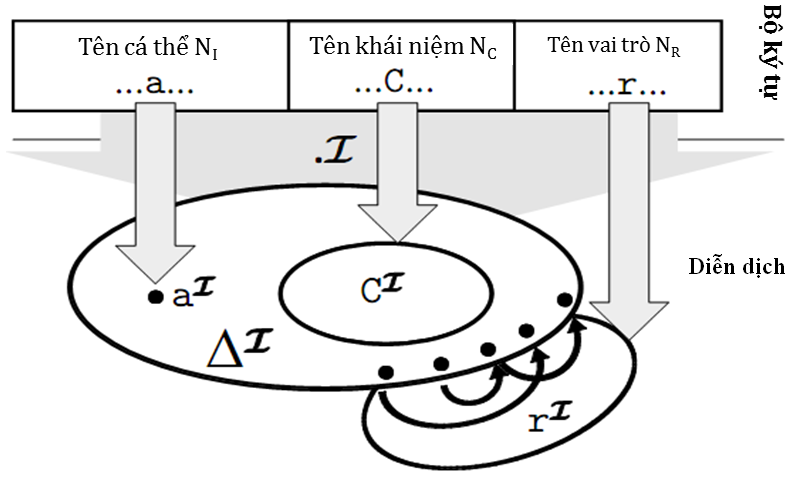
\includegraphics[scale=0.4]{NguNghia.png}
    \caption{Ngữ nghĩa của logic mô tả}\label{fig:Semantic}
  \end{center}
  
\end{figure}

Ngoài ra, ngữ nghĩa của các khái niệm phức có thể được xác định như Hình~\ref{fig:SemanticALC}.

\begin{figure}
  \begin{center}
    \begin{tabular}{|l c l|}
      \hline
      $\top^\mI$ &\!\!\!\!=\!\!\!\!& $\Delta^\mI$\\
      $\bot^\mI$ &\!\!\!\!=\!\!\!\!& $\emptyset$\\
      $\neg C^\mI$ &\!\!\!\!=\!\!\!\!& $\Delta^\mI \setminus C^\mI$\\
      $(C \mand D)^\mI$ &\!\!\!\!=\!\!\!\!& $C^\mI \cap D^\mI$\\
      $(C \mor D)^\mI$ &\!\!\!\!=\!\!\!\!& $C^\mI \cup D^\mI$\\
      $(\V r.C)^\mI$ &\!\!\!\!=\!\!\!\!& $\{x \in \Delta^\mI \mid \V y \mid \tuple{x, y} \in r^\mI \rightarrow y\in C^\mI\}$\\
      $(\E r.C)^\mI$ &\!\!\!\!=\!\!\!\!& $\{x \in \Delta^\mI \mid \E y \mid \tuple{x, y} \in r^\mI \wedge y\in C^\mI\}$\\
    
    \hline
    \end{tabular}
    \caption{Ngữ nghĩa các khái niệm phức của logic mô tả \ALC}\label{fig:SemanticALC}
  \end{center}
  
\end{figure}

Ta nói rằng $C^\mI$ là diễn giải của khái niệm $C$ trong diễn dịch $\mathcal{I}$ và $r^\mI$ là diễn giải của vai trò $r$ trong diễn dịch $\mI$. Nếu một đối tượng $x \in C^\mI$, lúc đó ta nói $x$ là một thể hiện của $C$ trong diễn dịch $\mI$.

Như đã đề cập trong phần giới thiệu, một cơ sở tri thức trong logic mô tả (knowledge base - KB) gồm có hai phần, bộ thuật ngữ (TBox) và bộ khẳng định (ABox), mỗi phần như vậy chứa tập các tiên đề. Dạng tiên đề tổng quát nhất của TBox được gọi là tiên đề bao hàm tổng quát.

\begin{Definition}\label{def:GCI}
Một \textnormal{tiên đề bao hàm tổng quát} (general concept inclusion - GCI) là một tiên đề có dạng $C \sqsubseteq D$, trong đó $C$ và $D$ là các khái niệm của \ALC.\myend
\end{Definition}

\begin{Definition}\label{def:TBox}
Một tập hữu hạn các tiên đề bao hàm tổng quát được gọi là một \textnormal{hộp thuật ngữ - TBox}.\myend
\end{Definition}

\begin{Definition}\label{def:ModelTBox}
 Một diễn dịch $\mI$ là một \textnormal{mô hình} của một tiên đề bao hàm tổng quát $C \sqsubseteq D$ nếu $C^\mI \subseteq D^\mI$; diễn dịch $\mI$ là mô hình của TBox $\mT$ nếu nó là mô hình của tất cả các tiên đề bao hàm tổng quát trong $\mT$.\myend
\end{Definition}

Đối với tiên đề tương đương dạng $C \equiv D$, chúng ta xem nó như là một dạng rút gọn của cặp tiên đề $C \sqsubseteq D$ và $D \sqsubseteq C$. Một tiên đề dạng $A \equiv C$, trong đó $A$ là một tên khái niệm, được gọi là một \textit{định nghĩa khái niệm}. 

Một TBox $\mathcal{T}$ được gọi là \textit{khả định nghĩa} nếu nó chỉ chứa các định nghĩa khái niệm kèm theo những ràng buộc sau:
\begin{itemize}
  \item $\mT$ chứa nhiều nhất một định nghĩa cho một tên khái niệm.
  
  \item $\mT$ có cấu trúc chuỗi không vòng, nghĩa là với bất kỳ một định nghĩa khái niệm $A$ nào trong $\mT$ không được tham chiếu trực tiếp cũng như gián tiếp tới chính khái niệm $A$.
\end{itemize}

Một TBox khả định nghĩa được gọi là một TBox có \textit{cấu trúc chuỗi không vòng}. Với một TBox $\mT$ khả định nghĩa, các tên khái niệm xuất hiện trong vế trái của định nghĩa được gọi là \textit{khái niệm định nghĩa}. những tên khái niệm khác được gọi là \textit{khái niệm nguyên thủy}. Đối với những TBox khả định nghĩa thì diễn giải của các khái niệm định nghĩa được xác định duy nhất thông qua diễn giải của các khái niệm nguyên thủy và vai trò nguyên thủy. Nhìn từ quan điểm tính toán, TBox khả định nghĩa được quan tâm nhiều vì nó cho phép sử dụng các kỹ thuật suy luận đơn giản \cite{ref:Baader00} và chúng ta sẽ thấy rằng suy luận trên các TBox khả định nghĩa thường có độ phức tạp thấp hơn nhiều so với suy luận trên TBox tổng quát.

Một ABox có thể chứa hai dạng tiên đề, dạng thứ nhất là tiên đề khẳng định khái niệm, nghĩa là khẳng định một cá thể là thể hiện của một khái niệm đã cho; dạng thứ hai là tiên đề khẳng định vai trò, nghĩa là khẳng định một cặp cá thể là thể hiện của một vai trò đã cho.

\begin{Definition}\label{def:Assertion}
Cho $N_I$ là một tập hợp các tên cá thể. Một \textnormal{tiên đề khẳng định cá thể} là một tiên đề có dạng $C(x)$ (gọi là \textnormal{tiên đề khẳng định khái niệm}) hoặc $r(x, y)$ (gọi là \textnormal{tiên đề khẳng định vai trò}), trong đó $C$ là một khái niệm của \ALC, $r$ là một vai trò của \ALC\ và $x, y$ là các tên cá thể.\myend
\end{Definition}

\begin{Definition}\label{def:ABox}
Một tập hữu hạn các tiên đề khẳng định cá thể được gọi là một \textnormal{hộp khẳng định - ABox}.\myend
\end{Definition}

\begin{Definition}\label{def:ModelABox}
Một diễn dịch $\mI$ là mô hình của tiên đề $C(x)$ nếu $x^\mI \in C^\mI$; diễn dịch $\mI$ là mô hình của tiên đề $r(x, y)$ nếu $\tuple{x, y} \in r^\mI$; diễn dịch $\mI$ là mô hình của ABox $\mA$ nếu nó là mô hình của mọi tiên đề trong $\mA$.\myend
\end{Definition}

Lưu ý, một vài tài liệu ký hiệu các tiên đề khẳng định cá thể trong ABox là $x:C$ thay cho $C(x)$ và $\tuple{x, y}:r$ thay cho $r(x, y)$.

\begin{Definition}\label{def:KB}
Một \textnormal{cơ sở tri thức} (knowledge base - KB) là một cặp $\tuple{\mathcal{T, A}}$, trong đó $\mT$ là một TBox và $\mA$ là một ABox. Một diễn dịch $\mI$ là mô hình của cơ sở tri thức $\mathcal{K=\tuple{T,A}}$ nếu $\mI$ là mô hình của cả $\mT$ và $\mA$.\myend
\end{Definition}

Chúng ta viết $\mI \models \mathcal{K}$ (tương ứng $\mI \models \mT$, $\mI \models \mA$ và $\mI \models \varphi$) để ký hiệu cho $\mI$ là mô hình của $\mathcal{K}$ (tương ứng TBox $\mT$, ABox $\mA$ và tiên đề $\varphi$).

\subsection{Các bài toán suy luận}\label{subsec:ReasonProb}

Trong mục này, chúng ta định nghĩa các bài toán suy luận dựa trên cơ sở tri thức bao gồm một TBox và một ABox~\cite{ref:Baader01, ref:Baader02, ref:Tobies}. Tiếp đó, chúng ta sẽ xem xét các trường hợp đặc biệt trong đó TBox/ABox rỗng hoặc trường hợp TBox thỏa mãn thêm một số ràng buộc, chẳng hạn như tính khả định nghĩa.

\begin{Definition}\label{def:ReasonPro}
Cho một cơ sở tri thức $\mathcal{K = \tuple{T,A}}$, trong đó $\mT$ là một TBox và $\mA$ là một ABox.
  \begin{itemize}
    \item Cơ sở tri thức $\mathcal{K}$ được gọi là \textnormal{nhất quán} nếu nó có mô hình.

    \item Khái niệm $C$ được gọi là \textnormal{thỏa mãn dựa trên $\mathcal{K}$} nếu tồn tại một mô hình $\mI$ của $\mathcal{K}$ sao cho $C^\mI \neq \emptyset$. Lúc đó $\mI$ cũng được gọi là \textnormal{mô hình} của $C$ dựa trên $\mathcal{K}$.

    \item Khái niệm $D$ \textnormal{bao hàm} khái niệm $C$ dựa trên $\mathcal{K}$ (viết là $\mathcal{K} \models C \sqsubseteq D$) nếu $C^\mI \subseteq D^\mI$ với mọi mô hình $\mI$ của $\mathcal{K}$.

    \item Hai khái niệm $C$ và $D$ \textnormal{tương đương nhau} dựa trên $\mathcal{K}$ (viết là $\mathcal{K} \models C \equiv D$) nếu $C^\mI = D^\mI$ với mọi mô hình $\mI$ của $\mathcal{K}$.

    \item Hai khái niệm $C$ và $D$ \textnormal{không giao nhau} dựa trên $\mathcal{K}$ nếu $C^\mI \cap D^\mI = \emptyset$ với mọi mô hình $\mI$ của $\mathcal{K}$.

    \item Cá thể $a$ là \textnormal{thể hiện của khái niệm} $C$ dựa trên $\mathcal{K}$ (viết là $\mathcal{K} \models C(a)$) nếu $a^\mI \in C^\mI$ với mọi mô hình $\mI$ của $\mathcal{K}$.

    \item Cặp cá thể $a, b$ là \textnormal{thể hiện của vai trò} $r$ dựa trên $\mathcal{K}$ (viết là $\mathcal{K} \models r(a,b)$) nếu $\tuple{a^\mI, b^\mI} \in r^\mI$ với mọi mô hình $\mI$ của $\mathcal{K}$.\myend
  \end{itemize}
\end{Definition}

Đối với logic mô tả \ALC, các bài toán suy luận được định nghĩa ở trên có thể chuyển thành bài toán nhất quán của một cơ sở tri thức. Chẳng hạn, $\mathcal{\tuple{T, A}} \models C(a)$ nếu và chỉ nếu $\tuple{\mT, \mA \cup \neg C(a)}$ không nhất quán.

\begin{proposition}\label{pro:ReduceSubsumption}
\textbf{(Chuyển đổi thành bài toán bao hàm)} Cho hai khái niệm $C$ và $D$, ta có:
\begin{enumerate}
  \item $C$ không thỏa $\Leftrightarrow$ $C$ được bao hàm bởi $\bot$;
  \item $C$ và $D$ tương đương nhau $\Leftrightarrow$ $C$ được bao hàm bởi $D$ và $D$ được bao hàm bởi $C$;
  \item $C$ và $D$ không giao nhau $\Leftrightarrow$ $C \mand D$ được bao hàm bởi $\bot$.\myend
\end{enumerate}
\end{proposition}

\begin{proposition}\label{pro:ReduceUnSat}
\textbf{(Chuyển đổi thành bài toán không thỏa)} Cho hai khái niệm $C$ và $D$, ta có:
\begin{enumerate}
  \item $C$ bao hàm bởi $D$ $\Leftrightarrow$ $C \mand \neg D$ không thỏa;
  \item $C$ và $D$ tương đương nhau $\Leftrightarrow$ cả $(C \mand \neg D)$ và $(\neg C \mand D)$ không thỏa;
  \item $C$ và $D$ không giao nhau $\Leftrightarrow$ $C \mand D$ không thỏa.\myend
\end{enumerate}
\end{proposition}

\section{Mở rộng của logic mô tả \ALC}
Như đã giới thiệu, logic mô tả \ALC\ là một trong những logic mô tả cơ bản nhất, nó được mở rộng từ logic mô tả \AL\ (logic \AL\ là logic giống như \ALC\ nhưng không cho phép tạo tử phủ định áp dụng trên một khái niệm bất kỳ mà chỉ cho phép tạo tử phủ định áp dụng trên các khái niệm nguyên tử). Để đạt được khả năng biểu diễn tốt hơn, người ta thực hiện việc mở rộng logic mô tả \ALC\ nhằm đáp ứng được những nhu cầu trong thực tế bao gồm những mở rộng về hạn chế số lượng không định tính, hạn chế số lượng định tính, vai trò nghịch đảo, vai trò bắc cầu, phân cấp vai trò, tính định danh, \ldots

\subsection{Logic mô tả \ALCN}
Tạo tử \textit{hạn chế số lượng không định tính} (\textit{unqualified $\mathcal{N}$umber restrictions}), ký hiệu bởi chữ cái $\mathcal{N}$ và được viết là $\geq n r$ (hạn chế ít nhất) và $\leq n r$ (hạn chế nhiều nhất), trong đó $n$ là một số nguyên không âm. Với những hạn chế này, ngữ nghĩa của hàm diễn dịch sẽ như sau:
$$(\geq n r)^\mI = \{x \in \Delta^\mI \mid \#\{y \mid \tuple{x, y} \in r^\mI\} \geq n \}\footnote{$\#\Gamma$ ký hiệu cho lực lượng của tập hợp $\Gamma$}$$
và 
$$(\leq n r)^\mI = \{x \in \Delta^\mI \mid \#\{y \mid \tuple{x, y} \in r^\mI\} \leq n \}$$

Như vậy, với tính chất hạn chế số lượng không định tính, chúng ta có thể mô tả số lượng các mối quan hệ theo dạng đã chỉ ra mà các cá thể phải thỏa mãn.

Với tạo tử hạn chế số lượng, chúng ta có thể xây dựng khái niệm để biểu diễn cho phát biểu ``\textit{những người có \textbf{nhiều nhất một người con} hoặc có \textbf{ít nhất là ba người con} và trong số ba người con đó có người là con gái.}'' như sau:
$$\mathsf{Person \mand (\leq 1\ hasChild \mor (\geq 3\ hasChild \mand \E hasChild.Female))}.$$

Tương tự như vậy, chúng ta muốn đưa ra khái niệm để biểu diễn cho phát biểu ``\textit{con người có thể kết hôn với \textbf{nhiều nhất một người khác}}'' bằng cách như sau:
$$\mathsf{Person \sqsubseteq\ \leq 1\, marriedTo},$$
và chúng ta cũng có thể định nghĩa khái niệm $\mathsf{HappyMan}$ với phát biểu ``\textit{người đàn ông hạnh phúc là người đàn ông kết hôn với bác sĩ, có \textbf{ít nhất là hai con}, \textbf{nhiều nhất là bốn con} và các con đều là bác sĩ hoặc giáo sư}'' như sau:
\[
  \begin{array}{r c l}
     \mathsf{HappyMan} & \equiv & \mathsf{Human \mand \neg Female \mand (\E marriedTo.Doctor)\, \mand}\\
     & & \mathsf{\geq 2\,hasChild\, \mand \leq 4\,hasChild}\\
     & & \mathsf{(\V hasChild.(Doctor \mor Professor))\, \mand}
  \end{array}
\]
\subsection{Logic mô tả \ALCQ}
Tạo tử \textit{hạn chế số lượng có định tính} (\textit{$\mathcal{Q}$ualified number restrictions}), ký hiệu bởi chữ cái $\mathcal{Q}$ và được viết là $\geq n r.C$ (hạn chế ít nhất) và $\leq n r.C$ (hạn chế nhiều nhất), trong đó $n$ là một số nguyên không âm, $C$ là một khái niệm. Với hạn chế số lượng có định tính, ngữ nghĩa của hàm diễn dịch như sau:
$$(\geq n r.C)^\mI = \{x \in \Delta^\mI \mid \#\{y \mid \tuple{x, y} \in r^\mI \wedge y \in C \} \geq n \}$$
và 
$$(\leq n r.C)^\mI = \{x \in \Delta^\mI \mid \#\{y \mid \tuple{x, y} \in r^\mI \wedge y \in C\} \leq n \}$$

Như vậy, chúng ta có thể mô tả các loại (định tính) cá thể quan hệ theo số lượng cho trước. 
\begin{Example}
Chẳng hạn như chúng ta có thể định nghĩa khái niệm $\mathsf{HappyMan}$ với phát biểu ``người đàn ông hạnh phúc là người đàn ông kết hôn với bác sĩ, có nhiều nhất là bốn con, các con đều là bác sĩ hoặc giáo sư trong đó có \textbf{ít nhất hai con là bác sĩ}'' như sau:
\[
  \begin{array}{r c l}
     \mathsf{HappyMan} & \equiv & \mathsf{Human \mand \neg Female \mand (\E marriedTo.Doctor)\, \mand}\\
     & & \mathsf{\leq 4\,hasChild \mand \V hasChild.(Doctor \mor Professor)\, \mand}\\
     & & \mathsf{\geq 2\,hasChild.Doctor}.
  \end{array}
\]
\end{Example}
\vspace{-5ex}
\myend

\subsection{Logic mô tả \ALCI}
Logic mô tả \ALCI\ cho phép sử dụng tạo tử \textit{nghịch đảo vai trò} (\textit{role $\mathcal{I}$nverse}) và ký hiệu bởi chữ cái $\mathcal{I}$. Một vai trò $r$ có vai trò nghịch đảo là $r^-$ với ngữ nghĩa được xác định như sau:
$$(r^-)^\mI = \{\tuple{y, x} \mid \tuple{x, y} \in r^\mI \}.$$

Với tạo tử nghịch đảo vai trò, chúng ta có thể xây dựng các vai trò nghịch đảo từ các vai trò đang có. Chẳng hạn, giả sử chúng ta có $\mathsf{hasChild}$ là vai trò đại diện cho một đối tượng này có con là đối tượng kia. Chúng ta có thể định nghĩa $\mathsf{hasParent = hasChild^-}$ là vai trò để đại diện cho một đối tượng này có bố mẹ là đối tượng kia.

\subsection{Logic mô tả $\mS$}
Một vai trò $r$ được gọi là \textit{vai trò bắc cầu} (\textit{transitive role}) nếu $r \circ r \sqsubseteq r$. Nghĩa là, với $r$ là vai trò bắc cầu, nếu ta có $\tuple{x, y} \in r^\mI$ và $\tuple{y, z} \in r^\mI$ thì $\tuple{x, z} \in r^\mI$.

Logic mô tả \ALC\ có các \textit{vai trò bắc cầu} (\textit{tran$\mS$itive roles}) được ký hiệu là $\mathcal{ALC}_{R^+}$. Để tránh việc phải viết các ký tự dài dòng, người ta sử dụng ký hiệu $\mS$~\cite{ref:Horrock00} để chỉ logic mô tả \ALC\ mở rộng thêm tạo tử vai trò bắc cầu. Trong logic $\mS$, gọi $N_T \subseteq N_C$ là tập các vai trò bắc cầu, lúc đó với mọi $r \in N_T$ ta có $r \circ r \sqsubseteq r$. 

Với tạo tử vai trò bắc cầu, chúng ta xét $\mathsf{hasDescendant}$ là vai trò để chỉ đối tượng này có con cháu là đối tượng kia. Rõ ràng, $\mathsf{hasDescendant}$ là vai trò bắc cầu. Vì nếu $\tuple{x,y} \in \mathsf{hasDescendant}$ và $\tuple{y, z} \in \mathsf{hasDescendant}$ thì $\tuple{x,z} \in \mathsf{hasDescendant}$. Nghĩa là nếu đối tượng $x$ có con cháu là đối tượng $y$ và đối tượng $y$ có con cháu là đối tượng $z$ thì đối tượng $x$ cũng có con cháu là đối tượng $z$. Lúc đó, để ký hiệu $\mathsf{hasDescendant}$ là vai trò bắc cầu, người ta viết $\mathsf{hasDescendant} \circ \mathsf{hasDescendant} \sqsubseteq \mathsf{hasDescendant}$. Tương tự như vậy, chúng ta có thể xây dựng $\mathsf{hasAncestor}$ là một vai trò bắc cầu để chỉ đối tượng này có tổ tiên là đối tượng kia và ký hiệu là $\mathsf{hasAncestor \circ hasAncestor \sqsubseteq hasAncestor}$.
\subsection{Logic mô tả \SH}
Logic $\mS$ có thêm tạo tử \textit{phân cấp vai trò} (\textit{$\mathcal{H}$ierarchies}) cho phép biểu diễn mối quan hệ phân cấp giữa các vai trò, gọi là tiên đề bao hàm vai trò và có dạng $r \sqsubseteq s$, trong đó $r$ và $s$ là các vai trò của logic mô tả \SH. Ngữ nghĩa của tiên đề bao hàm vai trò $r \sqsubseteq s$ được xác định là nếu $\tuple{x,y} \in r^\mI$ thì $\tuple{x,y} \in s^\mI$. Tập các tiêu đề bao hàm vai trò được gọi là một phân cấp vai trò.

\begin{Example}
Chúng ta có thể biểu diễn mối quan hệ phân cấp giữa vai trò $\mathsf{hasMother}$ (vai trò chỉ đối tượng này có mẹ là đối tượng kia) và vai trò $\mathsf{hasParent}$ (vai trò để chỉ đối tượng này có bố mẹ là đối tượng kia) như sau: $\mathsf{hasMother} \sqsubseteq \mathsf{hasParent}.$\myend
\end{Example}

\subsection{Logic mô tả \SI}
Logic môt tả \LogicS\ có thêm tạo tử \textit{nghịch đảo vai trò} (\textit{role $\mathcal{I}$nverse}). Cũng giống như tạo tử nghịch đảo thêm vào logic \ALC, nghịch đảo vai trò cho phép chúng ta xây dựng vai trò nghịch đảo từ những vai trò đã có. Tuy nhiên, đối với logic mô tả \LogicS, khi thêm tạo tử vai trò nghịch đảo sẽ có những phức tạp nảy sinh. Giả sử $r$ là một vai trò bắc cầu, lúc đó $r \circ r \sqsubseteq r$. Xét vai trò nghịch đảo của $r$ là $r^-$, ta cũng có $r^- \circ r^- \sqsubseteq r^-$. Hay nói cách khác, vai trò nghịch đảo của vai trò bắc cầu cũng là một vai trò bắc cầu. Điều này dễ dàng nhìn thấy thông qua ngữ nghĩa của vai trò bắc cầu $r$. Từ $\tuple{x, y} \in r^\mI$, $\tuple{y, z} \in r^\mI$ và $\tuple{x, z} \in r^\mI$, ta có $\tuple{y, x} \in (r^-)^\mI$, $\tuple{z, y} \in (r^-)^\mI$ và $\tuple{z, x} \in (r^-)^\mI$. Những vấn đề này sẽ gây ra những khó khăn nhất định cho việc suy luận thông qua thuật toán Tableaux vì cần phải đảm bảo tính bắc cầu cho các vai trò trong tập $N_T$ cũng như tính bắc cầu đối với các vai trò nghịch đảo của nó.

\begin{thebibliography}{10}

\bibitem{ref:Baader00}
F. Baader, D. Calvanese and D. L. McGuinness, D. Nardi, P. F. Patel-Scheider (Edt), The Description Logic Handbook: Theory, Implementation, and Applications, $2^{nd}$ edition, 2007.

\bibitem{ref:Baader01}
F. Baader and U. Sattler, An Overview of Tableau Algorithms for Description Logics, Studia Logica, Volume 69, Pages: 5--40, Springer, 2001.

\bibitem{ref:Baader02}
F. Baader, J. Hladik, C. Lutz and F. Wolter, From Tableaux to Automata for Description Logics, Fundamenta Informaticae, Volumn 57, Pages: 1--33, 2003.

\bibitem{ref:Brachman}
R. J. Brachman and J. G. Schmolze, An Overview of  the  \textsc{KL-one} Knowledge  Representation System, Cognitive Science, Vol 9, Pages: 171--216, 1985.

\bibitem{ref:Calvan}
D. Calvanese, M. Lenzerini and D. Nardi, Description Logics for Conceptual Data Modeling, Logics for Databases and Information Systems, Kluwer Academic Publisher, 1998.

\bibitem{ref:Horrock00}
I. Horrocks and U. Sattler, A Description Logic with Transitive and Inverse Roles and Role Hierarchies, Journal of Logic and Computation, Volumn 9(3), Pages: 385--410, 1999.

\bibitem{ref:Horrock01}
I. Horrocks, U. Sattler and S. Tobies, A $\textsc{PSPace}$-Algorithm for Deciding $\mathcal{ALCNI}_{\mathcal{R}^+}$-Satisfiability, LTCS-Report 98-08, 2000.

\bibitem{ref:Sahoo}
S. S. Sahoo and K. Thirunarayan, Tableau Algorithm for Concept Satisfiability in Description Logic $\mathcal{ALCH}$, TR-2009-07, 2009.

\bibitem{ref:Schimidt}
M. Schmidt-Schau\ss and G. Smolka, Attributive Concept Descriptions with Complements, Artificial Intelligence, Volumn 48, Pages: 1--26, Elsevier, 1991.

\bibitem{ref:Tobies}
S. Tobies, Complexity Results and Practical Algorithms for Logics in Knowledge Representation, Diploma Thesis, 2001.

\end{thebibliography}
\end{document}